\section{Threat Model and Objectives}
\label{sec:threat}

\begin{figure}[t]
\centering
\IfFileExists{figures/fig_observation.pdf}{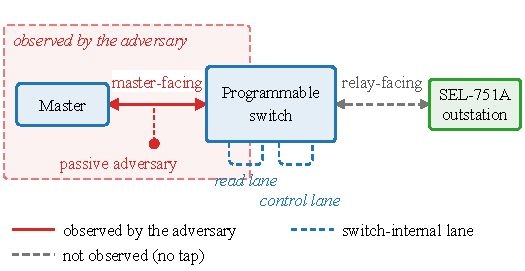
\includegraphics{figures/fig_observation}}{\figplaceholder{Observation model: master, observed master-facing link, programmable switch, relay-facing link (not observed), SEL-751A outstation.}}
\caption{Observation model. The adversary sees only the master-facing link (shaded); the relay-facing
  link and the switch-internal lanes (dashed) are observed by neither the adversary nor us.}
\label{fig:observation}
\end{figure}

\textbf{The adversary.} We assume a passive observer on the master-facing link, the adversary of
the fingerprinting attack we defend against~\cite{formbyWhosControlYour2016}.
Figure~\ref{fig:observation} shows where it sits. It records TCP and IP headers, segment sizes
and arrival times. It does not modify or inject packets, compromise the master or the outstation,
control the switch, or read the switch's internal state. It does not see the relay-facing link, which in our deployment is inside the switch with no tap
on it, and it does not see physical breaker motion.

Because DNP3 carries no transport security by default, we assume the traffic is
unencrypted~\cite{eastTaxonomyAttacksDNP32009}, so the observer also reads the DNP3 function
codes directly. An adversary that probes, injects, or otherwise acts on the network is out of scope. The
passive observer is the setting the traffic-obfuscation work we build on also targets.

\textbf{What the adversary is looking for.} Reconnaissance precedes the attacks that matter here. For example, false data injection
requires the attacker to know which devices it is dealing
with~\cite{liuFalseDataInjection2009}. Fingerprinting supplies that knowledge, and it does not
need the payload, because the timing of the exchange carries it. 

Following Formby et al.~\cite{formbyWhosControlYour2016}, two intervals are in scope. The first is
the CLRT of a READ or of the SELECT phase of a control, which measures the outstation's own
processing and which Section~\ref{sec:bg} shows carries the separation between the classes. The
second is the master-visible interval between an OPERATE's acknowledgment and its solicited
response. The adversary also sees the request-to-acknowledgment interval, whose median is 0.56~ms
on this device; the mechanism does not target it, and we report it as measured.

Our own observation is narrower than the adversary's in one direction and wider in none. Every
quantity we measure is one of three packet timestamps on the master-facing link: the request, the
acknowledgment and the response. The instants at which the switch releases a packet, and every
event on the relay-facing link, were not captured. Where the paper names them they come from the
configuration, and we say so.



The second interval deserves a careful statement, because it is easy to claim more for it than we
can support. Formby et al.\ estimate the time a device physically takes to complete an operation. However,
they do so from a sequence-of-events timestamp carried inside the outstation's application
payload, and their alternative estimate from packet arrival times produced no usable
result~\cite{formbyWhosControlYour2016}.  The interval we measure is a packet-timing feature of the solicited control response. It is not physical actuation time, and we do not measure physical actuation time anywhere. We
also make no claim about the payload-timestamp feature, which a mechanism that moves packets
without editing bytes could not affect in any case.

That narrower reading is still worth defending, because the interval separates the two classes on
its own and Section~\ref{sec:eval:ro3} shows an adversary recovering 0.651 balanced accuracy from
exactly that kind of difference. RO2 therefore asks whether the interval becomes a policy value,
not whether physical timing is concealed.

\textbf{What our evaluation actually separates.} Device fingerprinting is the application that
motivates the work. What we evaluate is narrower, and we keep the two apart throughout. Our
testbed has one outstation, so there is no second device to confuse it with and no device
identification to measure. What we measure is whether the timing of an exchange still reveals
\emph{which class of transaction} it was, on that one device. That is a three-class problem over
READ, SELECT and OPERATE, so chance is 0.333 balanced accuracy.  A result here is therefore the suppression of a class-conditioned timing feature, and not a
demonstration that two devices become indistinguishable.

\textbf{Two adversaries, not one.} We evaluate two conditions and report both. The \emph{fixed}
adversary learns transaction classes from undefended traffic and applies that model unchanged once
the defense is deployed; because the profile is built before the defense is met, this is the
adversary the reconnaissance setting describes. The \emph{adaptive} adversary collects obfuscated traffic and retrains on it, which answers what
remains learnable once the defense is deployed: it recovers 0.651 balanced accuracy where the
fixed one is left at chance. It needs no access the fixed one lacks, since the same passive
observer sees obfuscated traffic and the plaintext function codes label it; the two are evaluation
conditions rather than two adversaries with different powers. Both are ours, chosen to bracket the
problem, and the second is the one that limits our claim.

\textbf{Research objectives.} To make the goal checkable, we state it as five properties. The
evaluation answers each in turn, and we reuse the labels throughout.
\begin{itemize}
  \item \textbf{RO1 (read timing).} The visible CLRT of READ and of the SELECT phase of SBO is a
    configurable policy value rather than the outstation's own processing signature.
  \item \textbf{RO2 (control timing).} The master-visible OPERATE response-to-ACK interval stays at a
    policy value while the relay-facing hold is drawn from a configured codebook of 2, 6 and
    12~ms.
  \item \textbf{RO3 (timing leakage).} The timing features carry less information about the
    transaction class, and a fixed adversary that trained on undefended traffic is reduced to
    approximately three-class chance, which for READ, SELECT and OPERATE is 0.333 balanced
    accuracy.
  \item \textbf{RO4 (release policy and coverage).} The release budget, the range of policies the
    mechanism can realize, the fraction of traffic it can cover, and the residual it leaves are
    characterized rather than assumed.
  \item \textbf{RO5 (cost and protocol preservation).} We measure the latency the mechanism costs and the
    frames and bytes it adds, and the external DNP3 workload still completes: every request is
    answered and every control operation returns a success status.
\end{itemize}

\textbf{What is out of scope.} Two boundaries follow from the model above and hold for every
result we report. The framework does not hide the DNP3 function codes, which stay in plaintext, so
RO3 concerns the timing channel and not the command semantics. It also forwards every packet at
its original size, so it adds no size or segmentation signature of its own, while the delays it
imposes are themselves observable: an adversary who can time packets can see that something is
holding them. Because the relay-facing link is not instrumented, as stated above, the
per-transaction hold drawn from the configured codebook of 2, 6 and 12~ms is configured rather
than observed, which is why RO2 is stated in terms of the master-visible interval alone.
